
\newpage
\section{In-house Algorithmic Profiling}
\label{sec:inhouse}

In this section, we discuss the design and implementation for in-house algorithmic profiling.
Under in-house setting, 
developers can conduct algorithmic profiling 
to detect previously unknown complexity problems before releasing their software, 
or developers could diagnose and fix complexity problems 
reported by users through bug databases.
%For both of these two cases, 
%run-time overhead is not a major concern. 


\subsection{Design}
To conduct algorithmic profiling~\cite{Aprof1,Aprof2,AlgoProf},
we first need to record input \textit{size} and \textit{cost} for different code constructs 
during multiple executions,
we then plot records from the same code construct with input size as x-axis and cost as y-axis, 
and finally, we infer a cost function of the input size by using 
statistical curve fitting~\cite{curve-fitting} 
or curving bounding~\cite{curve-bounding}. 
Code constructs could be loops~\cite{AlgoProf} and functions~\cite{Aprof1,Aprof2}. 
To design algorithmic profiling, we need to select 
suitable metrics for input size and cost. 


%\begin{figure*}
%\centering
%\subfloat[MySQL\#27287]{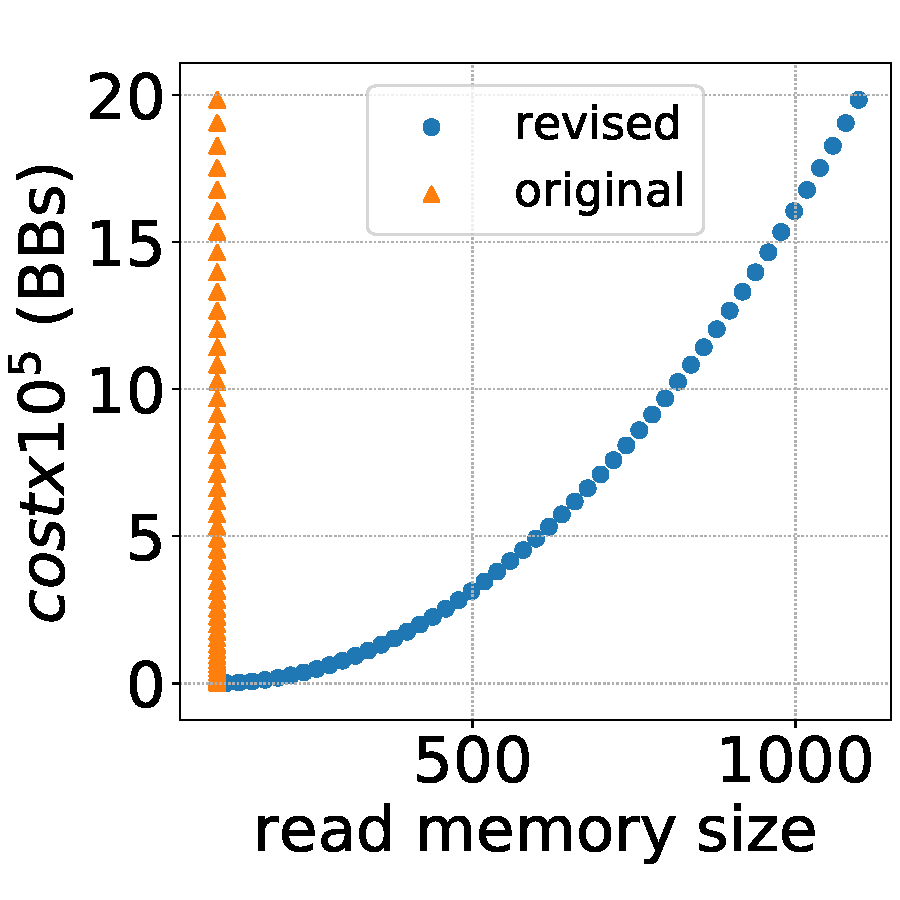
\includegraphics[width=0.24\linewidth]{figure/apache34464-line}\label{fig:mysql27287-line}} 
%\subfloat[GCC\#1687]{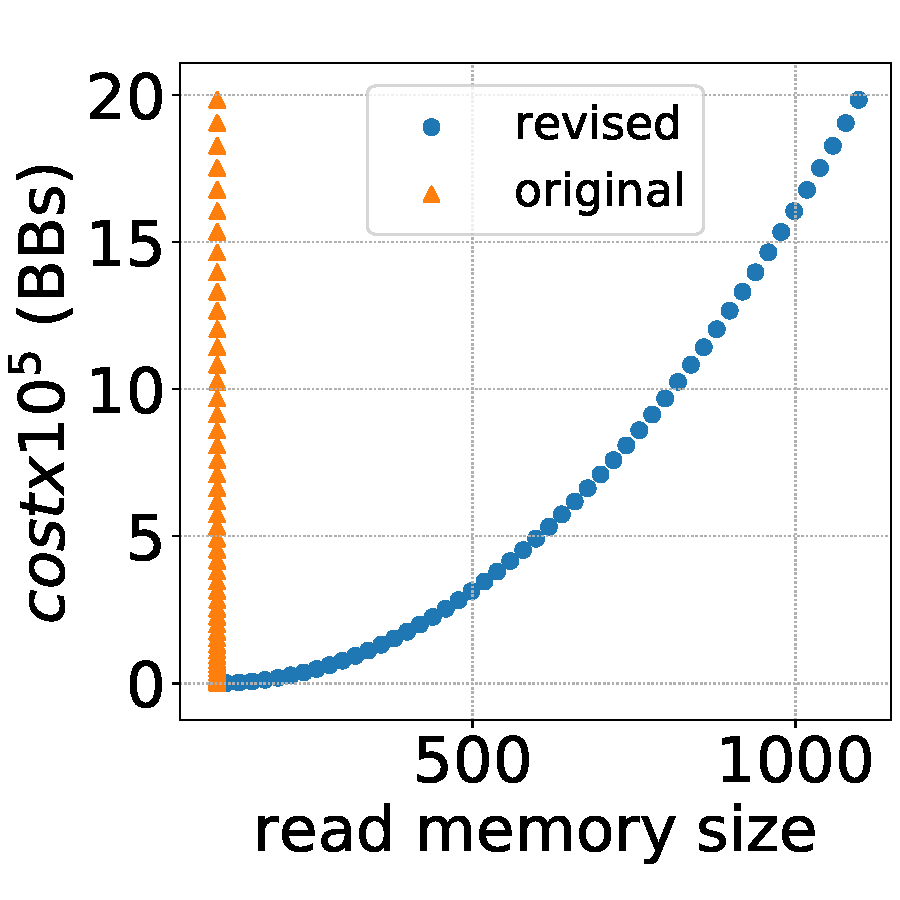
\includegraphics[width=0.24\linewidth]{figure/apache34464-line}\label{fig:jaccard}}
%\subfloat[fib]{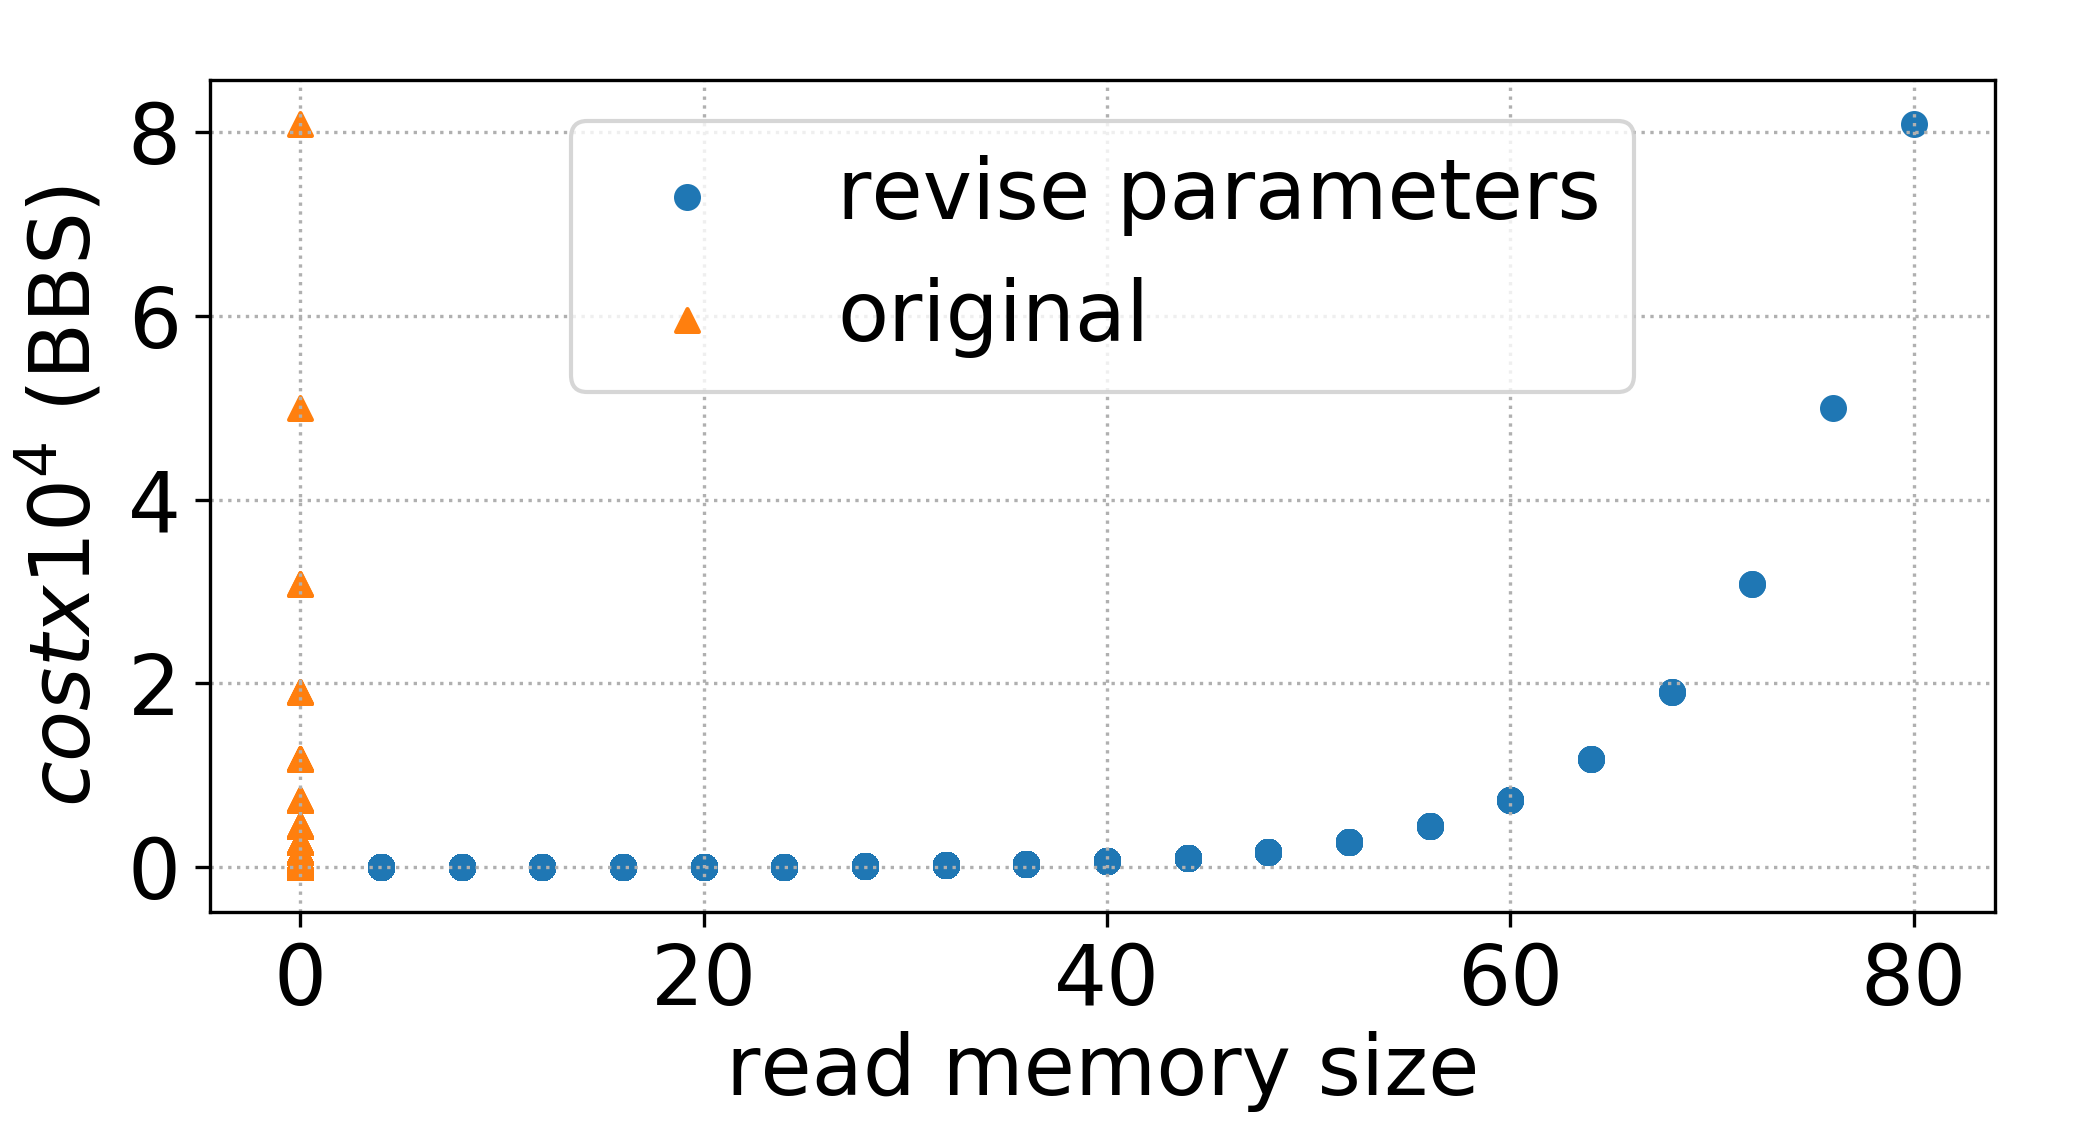
\includegraphics[width=0.24\linewidth]{figure/fib-line}\label{fig:fib-line}}
%\subfloat[Apache\#34464]{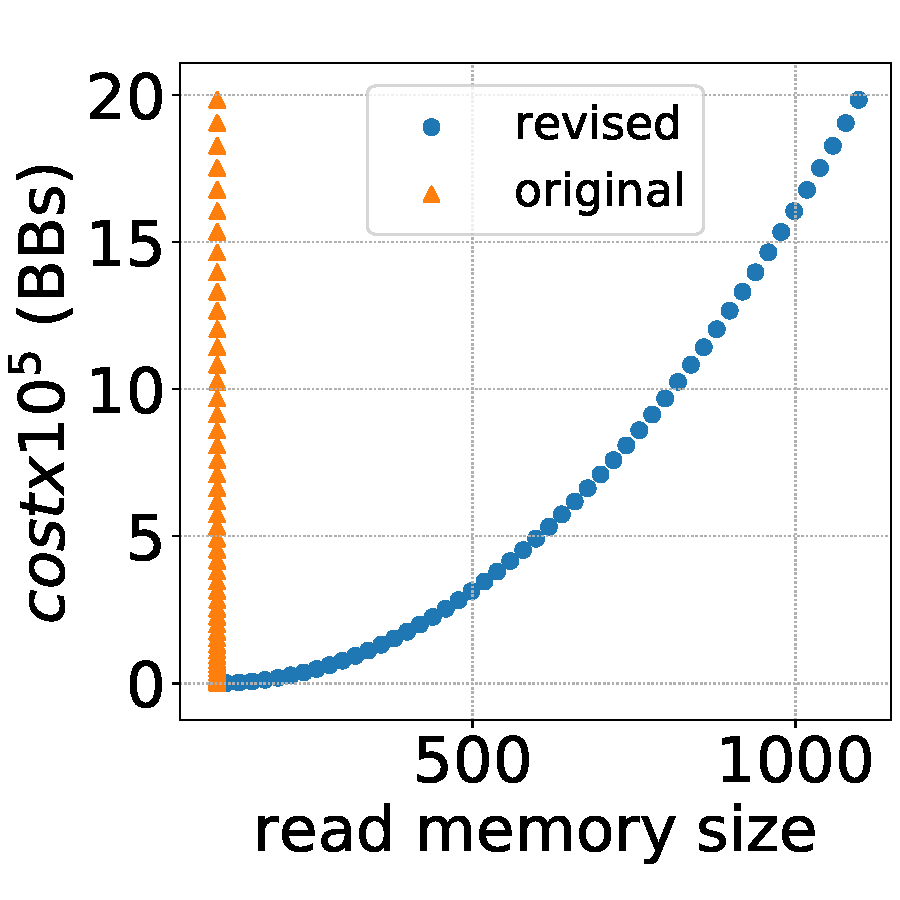
\includegraphics[width=0.24\linewidth]{figure/apache34464-line}\label{fig:apache34464-line}} \\ 
%\vspace{-0.1in}
%\caption{Cost function using RMS as input size. XXXXXX} 
%\label{fig:heat} 
%\end{figure*} 


%{{\bf{\underline{\textit{Input designs.}}}}
\subsubsection{How to design input metric?}
Many metrics can be used to measure input for a code construct. 
We discuss commonly used ones as follows.

\underline{\textit{Program input.}}
As discussed in Section~\ref{sec:process}, 
users tend to specify how to change the whole program 
input in order to describe the perceived complexity problem.
It is fairly easy to measure input size for the whole program based on users' report.
One way to measure input size for a code construct
is to simply use the input size of the whole program. 


\underline{\textit{Read memory size.}}
%Read memory size (RMS)is proposed as input size metric~\cite{Aprof1,Aprof2} . 
Read memory size (RMS) is defined as the number of distinct memory cells 
whose first access is read. 
RMS consider reads conducted by a code construct directly 
and reads conducted by 
functions called from the code construct. 


\begin{figure}
\centering
\subfloat[Inner loop]{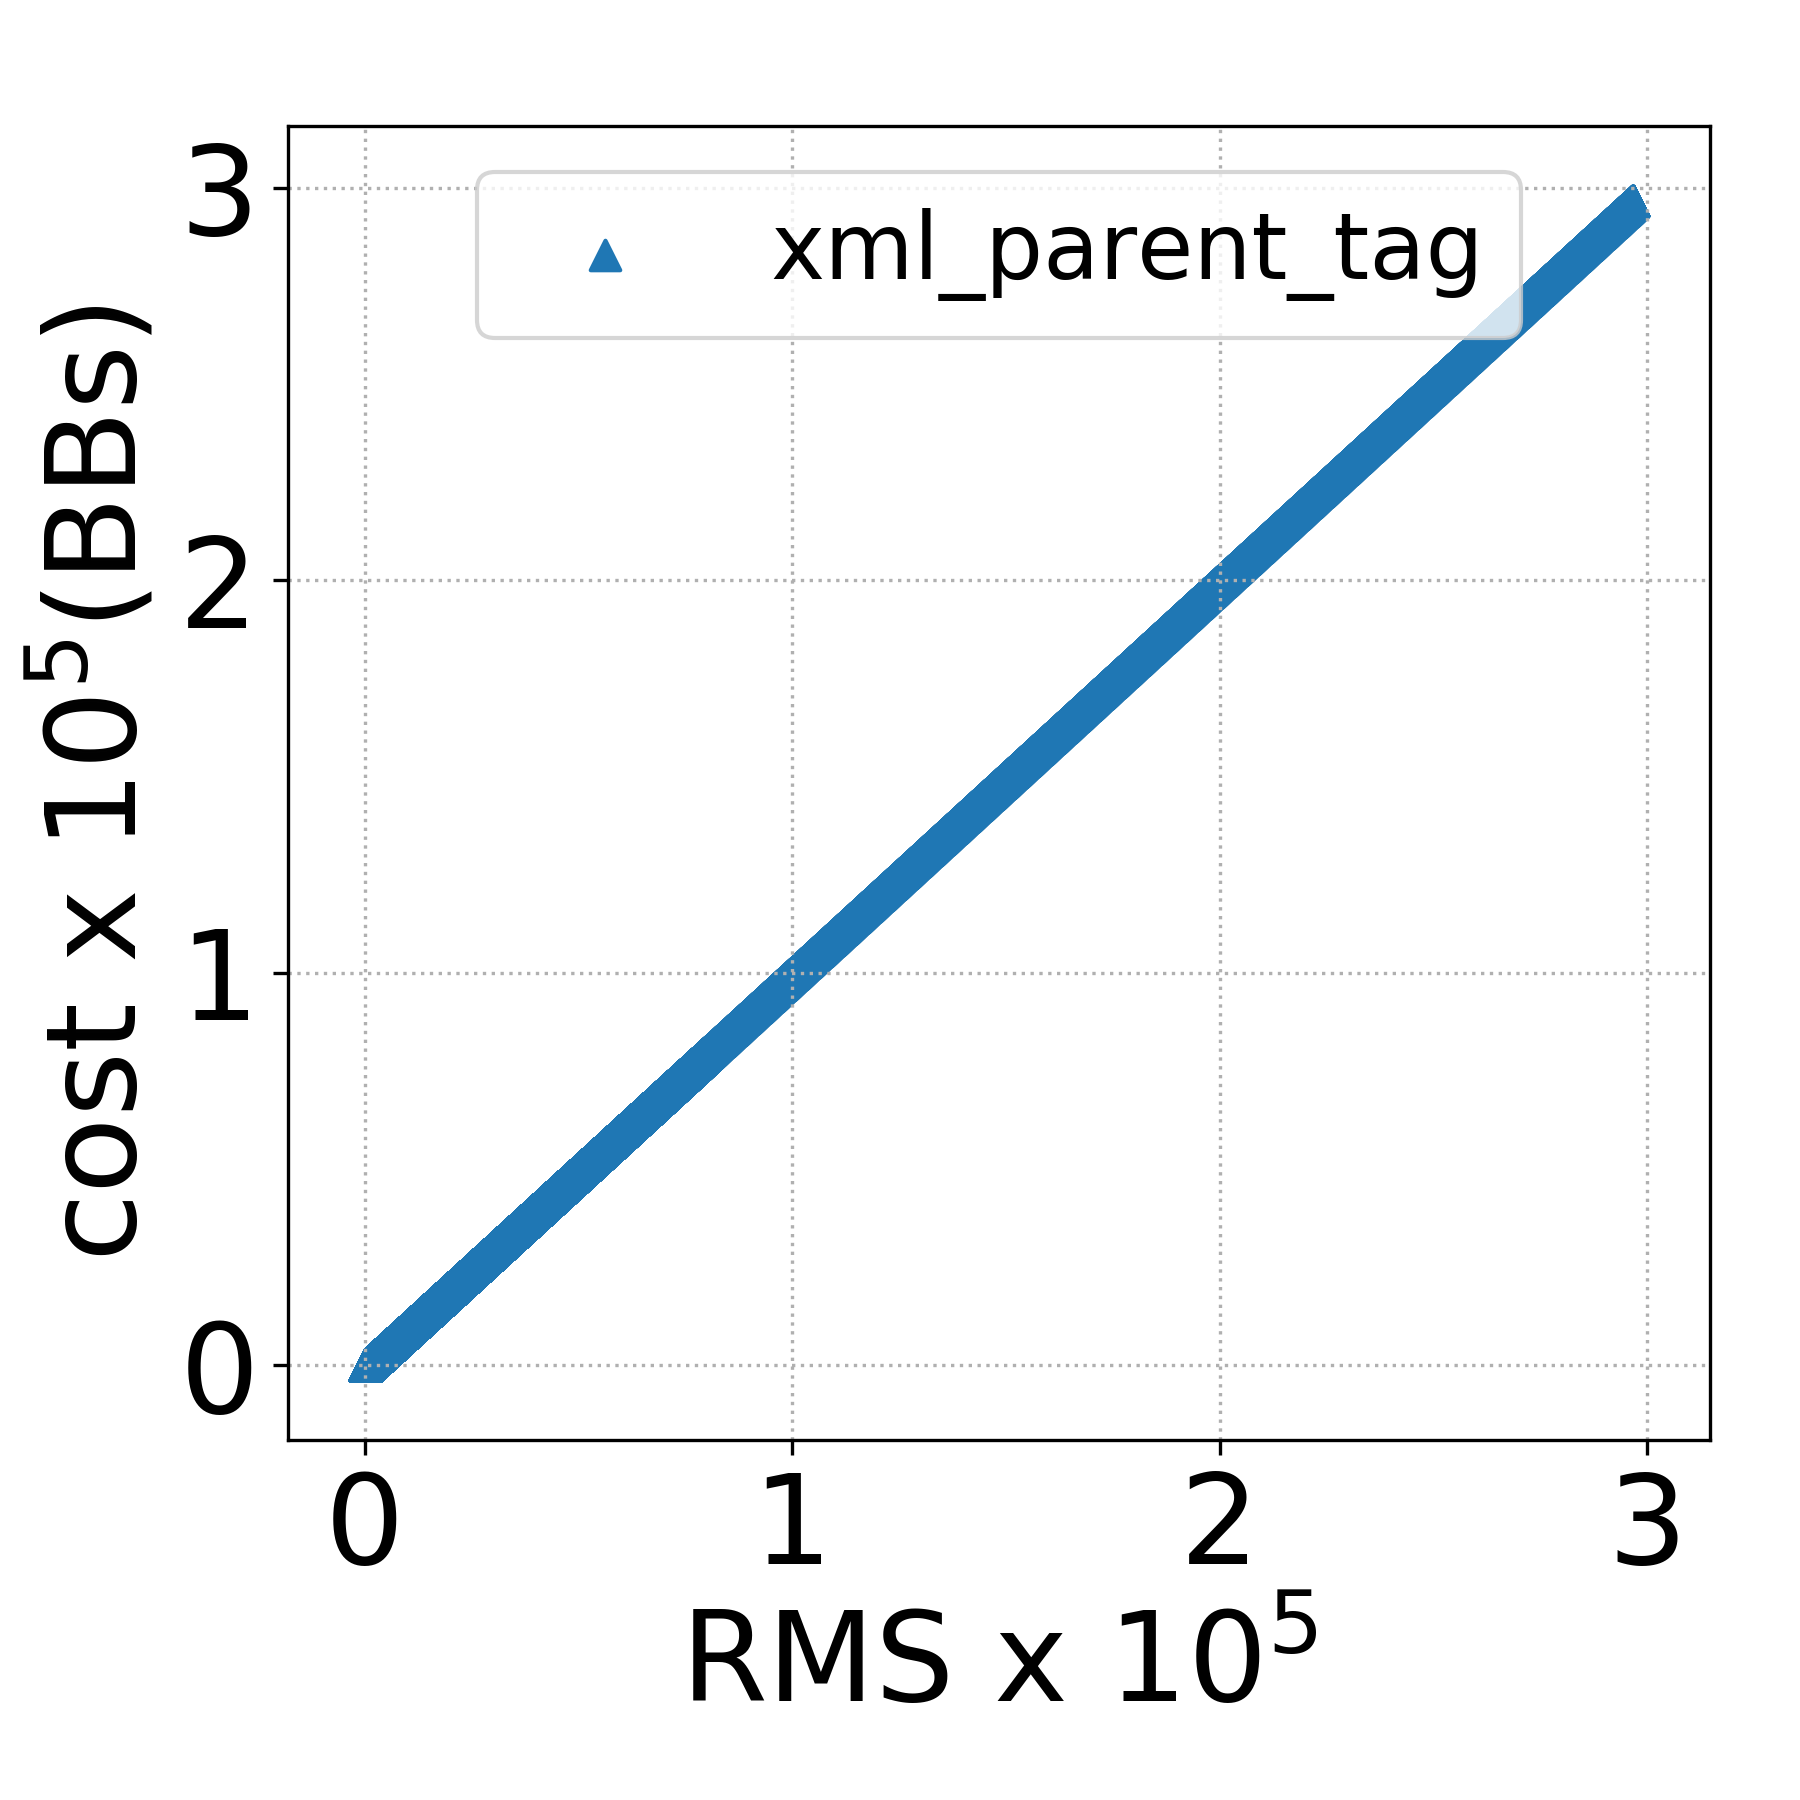
\includegraphics[width=0.42\linewidth]{figure/mysql27287-complexity-n}\label{fig:mysql27287-in}}
\subfloat[Outer loop]{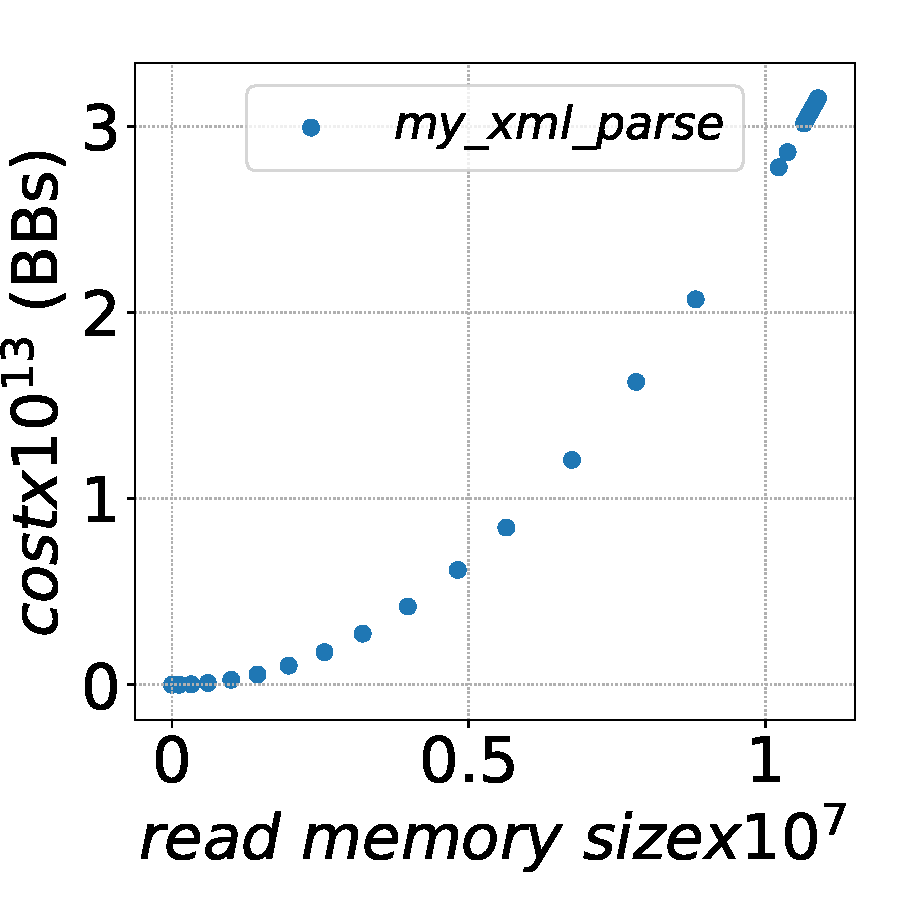
\includegraphics[width=0.42\linewidth]{figure/mysql27287-complexity-n-square}\label{fig:mysql27287-out}} \\ 
\vspace{-0.1in}
\caption{Inferred cost functions for MySQL\#27287 using RMS as input size.
\footnotesize{(\texttt{xml\_parent\_tag} is the function containing the inner loop, 
and \texttt{my\_xml\_parse} is the function containing the outer loop.)}} 
\label{fig:mysql27287-2} 
\end{figure} 

RMS is a generic metric for input size, 
and it can provide important input information for many complexity problems.   
For example, 
RMS for one execution of
the buggy loop in Figure~\ref{fig:mysql27287}
is roughly equal to 2 times the number of \texttt{XML\_NODE} 
accessed during the execution, 
because \texttt{level} field and \texttt{type} field of 
different \texttt{XML\_NODE}s are read in different loop iterations.
Although variable \texttt{p} and \texttt{level} are also read in each iteration,
RMS only considers distinct memory cells and 
only increases its value for the first read on these two variables in the first iteration. 
There is also an outer loop, 
and the outer loop invokes \texttt{xml\_parent\_tag} 
for every \texttt{XML\_NODE} contained
in the same array \texttt{items}. 
For that outer loop, its RMS is in linear relationship 
with the size of array \texttt{items}, 
since RMS only considers distinct memory cells 
and multiple reads conducted on the same memory 
cell of array \texttt{items} will not increase RMS. 
The inferred cost functions for the two functions 
containing the inner and the outer loop using RMS as input metric are shown 
in Figure~\ref{fig:mysql27287-2}.

{\underline{\textit{Data structure size.}}}
The number of accessed elements of a data 
structure could also be used to measure 
input size for a code construct~\cite{AlgoProf}. 
Commonly used data structures include linked lists and arrays.
Using data structure size can provide more semantic information for 
analyzed code constructs.
For example, if we focus on array \texttt{items}, 
the input size for both 
inner loop and outer loop of MySQL\#27287 is 
the number of accessed elements of array \texttt{items}.
Developers can clearly see that cost of each execution 
of the inner loop is in linear relationship with accessed elements, 
while the cost of the outer loop is in $O(N^2)$ relationship. 

In the reminder of this paper, we will focus on RMS as input metric. 
We skip the whole program input, 
because it is related to the input of a code construct in various ways.
Changing the whole program input may not change input sizes for 
all code constructs. 
Using the input size of the whole program as input metric for a code construct
may lead to incorrect profiling results. 
We also skip data structure size,
because it is not a generic metric. 
We need to design and implement extra static and dynamic techniques 
to identify data structures and figure out their sizes.


\subsubsection{How to design cost metric?}
There are also a lot of metrics which can be used to measure execution cost, 
such as the number of executed instructions, 
the time elapsed during execution,
the number of executed basic blocks (BBs), 
loop iteration, 
the number of recursive function call instances, and so on.

During our in-house technique design, 
we focus on the number of executed BBs. 
We do not use execution time, 
because when a code construct takes very little time,
using execution time may not provide an accurate measurement. 
We do not use the number of executed instructions, 
because this number is highly correlated with the number of BBs. 
Loop iteration and the number of recursive call instances could be used as estimates 
for the number of BBs. 
We do not use these two when designing in-house algorithmic profiling, 
but we will leverage them when building production-run techniques.  
 

\subsection{Implementation optimizations}

Aprof~\cite{Aprof1, Aprof2} is an algorithmic profiling tool built on Valgrind. 
Aprof uses RMS as input metric and executed BBs as cost metric.
Complexity information will be attributed to functions after profiling. 
We use LLVM framework to build an in-house algorithmic profiling tool.
Our tool building starts from the instrumentation algorithms used in aprof. 
We design a set of optimizations to reduce the runtime overhead, 
while providing accurate results.
In this section, we will first overview instrumentation algorithms in aprof firstly, 
and we will then discuss our designed optimizations. 

\subsubsection{Background}
To count executed BBs and RMS for each dynamic function call instance,
aprof runtime needs to maintain 5 global variables:
\texttt{cost}, 
tracking how many basic blocks are executed since the monitored program starts running, 
\texttt{count}, 
maintaining the current timestamp and increased by 1 after each function invocation, 
\texttt{ts}, 
a hash table containing the latest access timestamp for each memory cell,
\texttt{S}, 
a shadow stack tracking all active functions, 
and \texttt{top}, 
tracking the top of \texttt{S}.

Aprof instruments hook functions for 4 types of instructions: 
\texttt{call}, \texttt{return}, \texttt{read}, and \texttt{write}. 
When a function is invoked, 
\texttt{call} hook function will increment timestamp variable \texttt{count}
and grow the shadow stack \texttt{S} by incrementing \texttt{top}.
When a function returns,
\texttt{return} hook function will 
generate a log 
containing the returning function's RMS and executed BBs.
Since RMS also considers memory reads conducted by 
invoked callee functions, 
\texttt{return} hook function will add 
the RMS of the returning function to its caller on the stack. 
\texttt{read} hook function needs to query the hash table \texttt{ts} to decide  
whether to increment RMS for the function on top of the shadow stack \texttt{S}.
Both \texttt{read} and \texttt{write} 
hook function will update hash table \texttt{ts}
to maintain the latest access timestamp for an accessed memory cell. 


%{{{\bf{\underline{\textit{Aprof overview.}}}}
%\subsubsection{Background}
%Aprof uses the number of executed basic blocks as cost metric.
%To measure this number, aprof keeps a global counter \texttt{cost}, 
%which tracks how many basic blocks are executed since 
%starting the monitored program.
%To figure out whether a memory cell is accessed by the same function invocation before,
%aprof keeps another global counter \texttt{count}, 
%which tracks how many functions have been invoked.  
%Aprof maintains a shallow stack \texttt{S}, 
%which grows as the monitored program makes a function invocation, 
%and shrinks as the monitored program returns. 
%Aprof uses the third global variable \\texttt{top} to track the top of \texttt{S}.
%Aprof also maintains a hashmap \texttt{ts}, 
%which tracks latest access function for each distinct memory cell. 

%Aprof instruments 4 types of instructions: \texttt{call}, 
%\texttt{return}, \texttt{read}, and \texttt{write}. 
%When the monitored program makes a function call,
%aprof will increase \texttt{count} and \texttt{top} by 1.
%The new added stack entry will be initialized as follows, 
%\texttt{top.ts=count}, 
%\texttt{top.rms=0} and \texttt{top.cost=cost}.  
%Where the monitored program returns,
%aprof will create a log based on the content inside \texttt{S[top]}
%contribute the rms 
%of the returned function to its caller by doing \texttt{S[top-1].rms+=S[top].rms},
%and shrink the stack. 
%For a memory read on a cell \texttt{w},
%if \texttt{w}'s last access timestamp \texttt{ts[w]} is smaller 
%than the timestamp when the current function is invoked \texttt{S[top].ts},
%aprof will increase the RMS value for the current function.
%Since aprof will contribute an invoked function's rms to its caller, 
%aprof will also check active functions on the shadow stack and 
%decrease their RMS when necessary..   
%Aprof will set memory cell \texttt{w}'s latest access time 
%for all memory \texttt{read} and \texttt{write} on \texttt{w}.
%{\bf xxxx: these two parameters are very bad}
%{\bf remember to discuss how to change function to loop}

\subsubsection{Optimizations}
We design several optimizations to reduce the 
runtime overhead for our LLVM implementation from two aspects:
we try to reduce the number of instrumentation sites, 
and we try to accelerate hook functions. 

{\underline{\textit{Optimization 1}}
Our first optimization is designed to efficiently count the number of executed BBs.
Instead of incrementing a global counter by 1 inside every BB,
we apply an algorithm to decide where to update the BB counter and how to update the BB counter. 
The algorithm was originally designed to 
efficiently count edge events through selectively instrumenting counter 
on control flow graph~\cite{event-counting}. 
It has already been proved to be able to conduct path 
profiling efficiently~\cite{peter-ase,path-profiling}.

To apply the algorithm, we first instrument a local counter 
\texttt{local\_cost} at the beginning of each function
and initialize its value to be 0. 
We will add the value of \texttt{local\_cost} to the 
global counter \texttt{cost} before 
every function's return.
After that, we only need to consider where to update \texttt{local\_cost} 
within a single function.
We design and implement intra-procedural 
control flow analysis to achieve this.
Since the original algorithm is design to count events on edge,
we split each basic block into two and label event number to be 1 
for the edge connecting the two split basic blocks.  
We label event number to be 0 for all other edges. 
We calculate spanning tree for the new control flow graph. 
Edges not in the spanning tree are called chords.
We apply the depth-first search algorithm proposed in~\cite{event-counting} 
to calculate on which chords we should increase 
\texttt{local\_cost} and how much values 
we should add to \texttt{local\_cost}.


{\underline{\textit{Optimization 2}}
The second optimization tries to improve the performance of 
lookuping hash table \texttt{ts}, 
containing latest access timestamp for each memory cell.
For memory read, 
aprof needs to query \texttt{ts} and decide 
whether or not RMS should be incremented.
For memory read and write, 
aprof needs to update \texttt{ts} by using the current timestamp \texttt{count}
for accessed memory cells. 

Instead of using hash table, 
we use page table to contain timestamp information. 
To balance runtime overhead and memory overhead, 
we design a 4-layer page table for 32-bit programs.
We use 4 KB consecutive memory areas to hold pointers pointing to 
memory areas in the next layer 
or memory areas holding timestamps for memory cells. 
For a monitored 32-bit program, 
we need to calculate 4 addresses using bitwise operations 
and use the 4 addresses to refer each layer of the page table.  
For 64-bit programs, we use 6 layers.  


Compared with hash table, 
page page leverage locality of memory access 
and can lead 
to a better cache performance. 
To further improve performance, 
we add an extra variable to hold the pointer pointing 
to the last referred memory area holding timestamp.
For each memory read or write, 
we first check the saved pointer value can be used. 
We only conduct page table lookup, when the save value cannot be used. 

{\underline{\textit{Optimization 3}}
The third optimization targets reducing the number of instrumentation sites 
for \texttt{read} and \texttt{write}. 
We apply dominance analysis on 
control flow graph to achieve this.
For this optimization, we focus on stack memory cells holding 
scalar variables and only having \texttt{read} and \texttt{write} as uses 
(e.g. not having ``address of'' as uses).
We only focus on these memory cells,
because we want to avoid pointer alias analysis, 
which may potentially introduce inaccurate results. 
For a \texttt{read} instruction on one of these memory cells, 
if it is dominated by another \texttt{read} or \texttt{write} instruction 
on the same memory cell, we will skip to instrument this \texttt{read} instruction.
For a \texttt{write} instruction on one of these memory cells, 
if it is dominated by another \texttt{write} on the the same cell, 
we skip to instrument this \texttt{write}. 
{\bf xxx: add some numbers here}

 
{\underline{\textit{Optimization 4}}
For the last optimization, we apply inline functionality 
provide by LLVM to make all instrumented hook functions inline.


\subsection{Enhancing RMS}
There are two limitations in RMS. 
In this section, we will discuss how to augment  
RMS in order to address these two limitations.


\begin{figure}
\centering
\lstset{basicstyle=\ttfamily\fontsize{7}{8}\selectfont,
     morekeywords={+},keepspaces=true,numbers=left}
  \mbox{\lstinputlisting[mathescape,boxpos=t]{figure/fib.c}}
\caption{A recursive function to compute fibonacci number. 
(Execution time scales exponentially in the value of parameter \texttt{n}.) }
\vspace{-0.05in}
\label{fig:fib}
\vspace{-0.05in}
\end{figure}

\begin{figure}
\centering
\subfloat[fib]{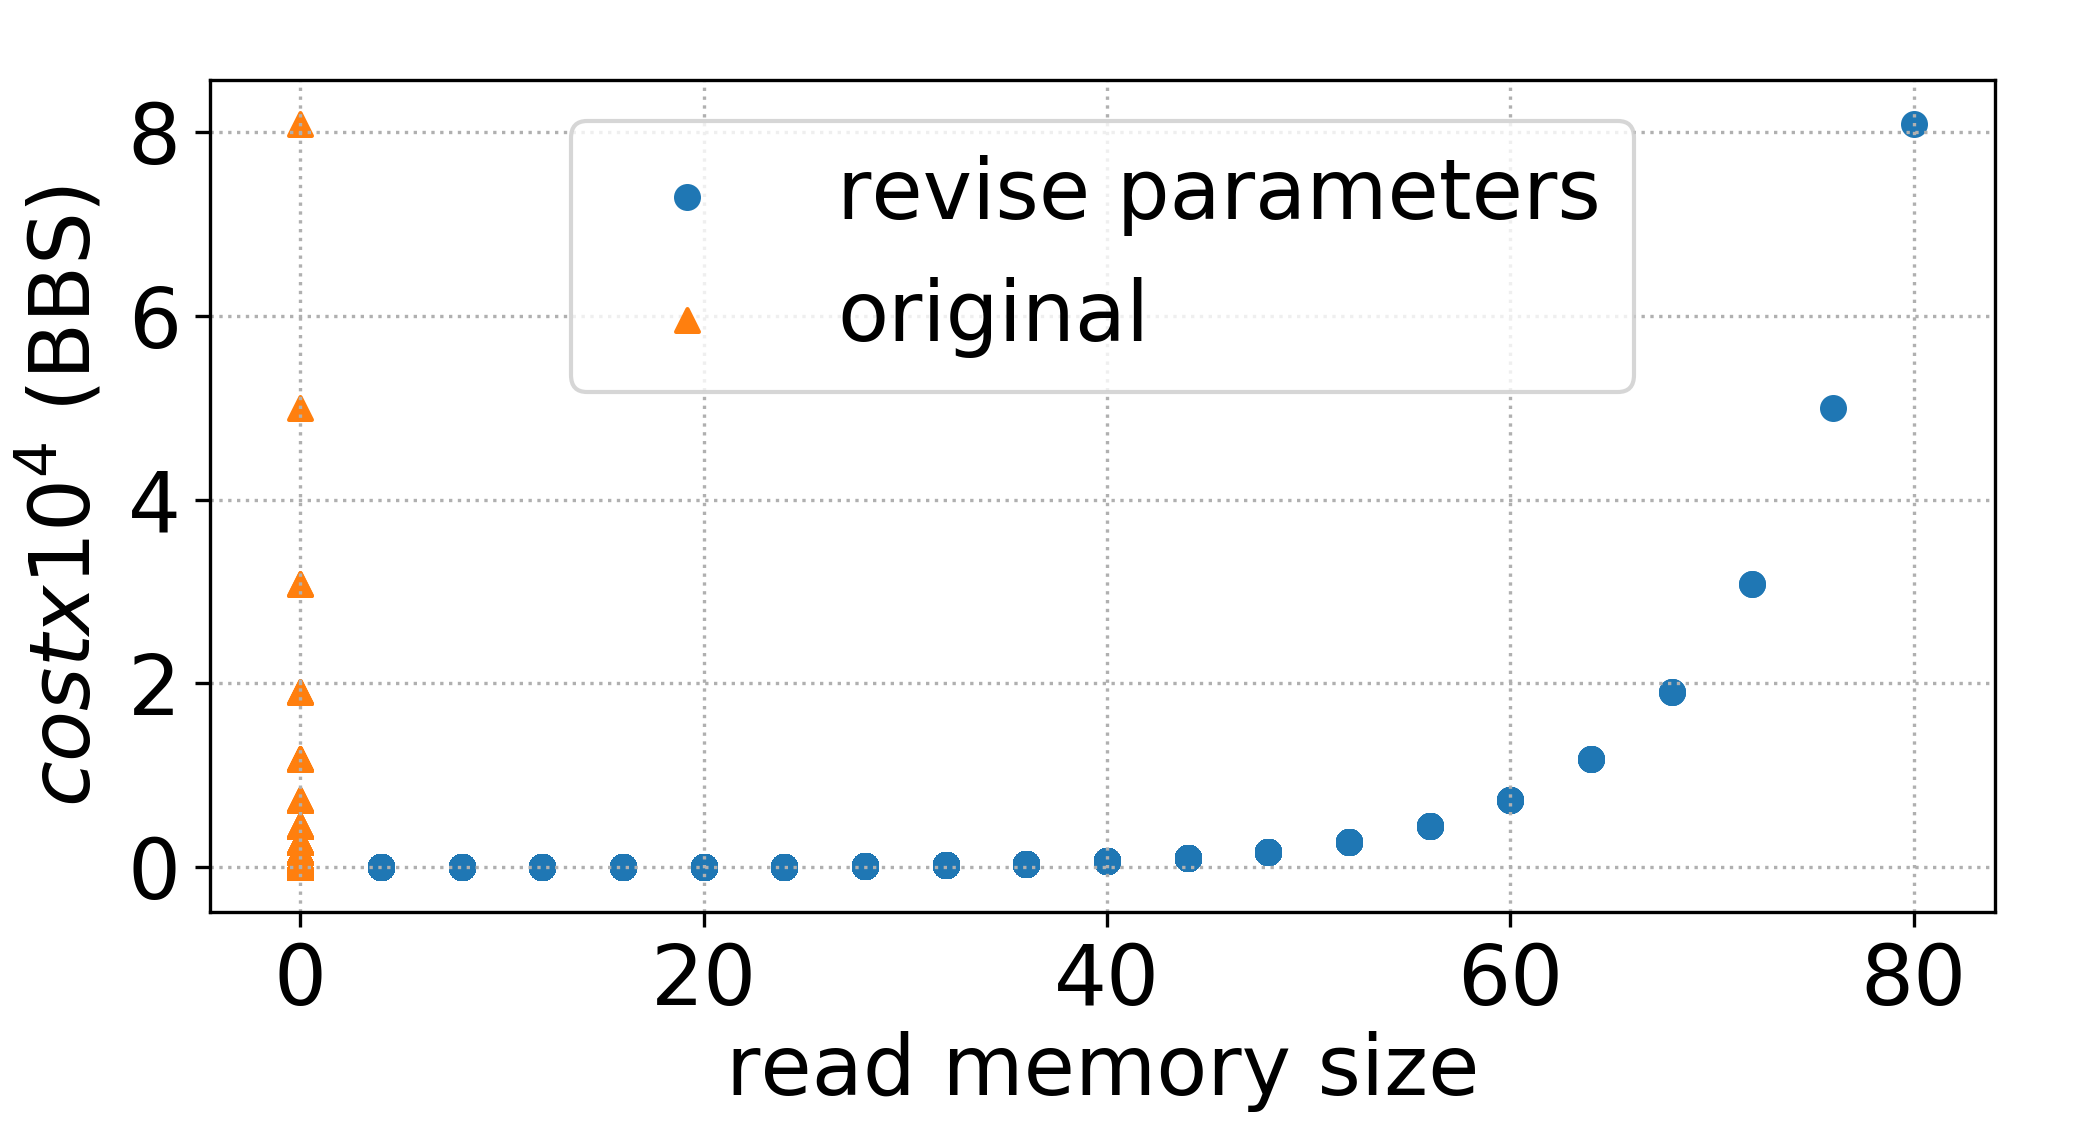
\includegraphics[width=0.42\linewidth]{figure/fib-line}\label{fig:fib-line}}
\subfloat[Apache\#34464]{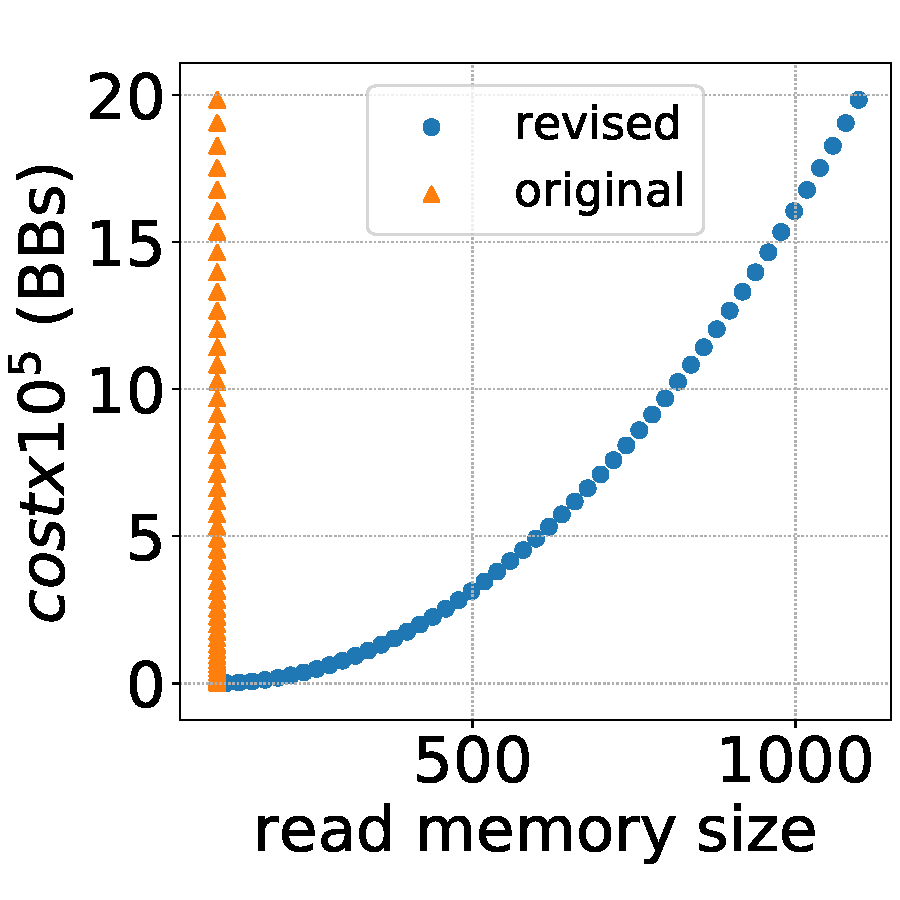
\includegraphics[width=0.42\linewidth]{figure/apache34464-line}\label{fig:apache34464-line}} \\ 
\vspace{-0.1in}
\caption{Cost function using RMS as input size. XXXXXX} 
\label{fig:heat} 
\end{figure} 

First, RMS cannot accurately measure input size for 
a recursive function
whose computation scales with the value of input parameter. 
Take the recursive function in Figure~\ref{fig:fib} as an example,
\texttt{fib} is to compute fibonacci number for parameter $n$.
For an invocation of \texttt{fib}, 
the first \texttt{read} on parameter $n$ will increment RMS.
However, after that, no matter how large $n$ is, RMS will not increment any more. 
This is because whenever \texttt{fib} recursively call itself on line 3, 
it needs to write parameter $n-1$ (or $n-2$) onto stack firstly, 
which means that the memory cell is accessed 
with \texttt{write} operation firstly.
To address this problem, when a function recursively call itself, 
we will increment RMS of the current function 
by the size of function call parameters. 
For example, when a call instance of $fib$ recursive calls itself 
($fib(n-1)$ or $fib(n-2)$) on line 3,
we will increment its RMS by 4.
The plots for $fib$ before and after algorithm 
adjustment is shown in Figure~\ref{fig:fib-line}.
Before adjustment, 
RMS will always be the same plotted 
as the vertical line on the left. 



\begin{figure}
\centering
\lstset{basicstyle=\ttfamily\fontsize{7}{8}\selectfont,
     morekeywords={+},keepspaces=true,numbers=left}
  \mbox{\lstinputlisting[mathescape,boxpos=t]{figure/apache34464.c}}
\caption{An Apache performance problem in $O(N^2)$ complexity. 
(Execution time scales polynomially in the number of characters read from  \texttt{getchar()}.) }
\vspace{-0.05in}
\label{fig:apache34464}
\vspace{-0.05in}
\end{figure}

Second, RMS does not consider inputs from I/O.
Buggy code fragment for Apache\#34463 is shown 
in Figure~\ref{fig:apache34464}.
The \texttt{while} loop on line 4 searches a string \texttt{source} for a target sub-string \texttt{target}.
If the \texttt{while} loop cannot find, 
a new character from I/O function \texttt{getchar()} 
on line 6 will be appended to string \texttt{source}, 
and the loop will search string \texttt{source} again from the beginning. 
The input size for this piece of codes depend on how many 
characters got from \texttt{getchar()}.
The computation scales polynomially as the input size.
Since all memory cells of string \texttt{source} are written 
firstly using return value of \texttt{getchar()}, 
no matter how many characters we get from \texttt{getchar()}, 
RMS of this piece of code only depends 
on the size of string \texttt{target}, 
variable \texttt{sourceLen} and variable \texttt{targetLen}.
To address this problem, 
we keep a list of I/O functions. 
When these functions are called, 
we will increment RMS for all 
functions active on the shadow stack. 
The plots for the function containing the buggy loop 
before and after algorithm adjustment is shown in Figure~\ref{fig:apache34464-line}.
Before adjustment, 
RMS will always be the same no 
matter how many characters received from \texttt{getchar()}. 


\subsection{Discussions}

RMS considers memory reads conducted by functions called from a code construct,
while it does not consider memory accesses 
by the same code construct from different executions.
Basically, RMS measures input size in a top-down view.
In the next section, we will discuss why it is difficult to apply sampling to RMS.

All the optimizations proposed in this section can reduce runtime overhead 
without changing profiling results.
Approximate algorithms could be explored to further reduce overhead. 
For example, in our current implementation, 
we use byte as unit for distinct memory cells.
We could explore to use larger units, like 4 bytes or 16 bytes. 
Using a larger unit can reduce both memory overhead and runtime overhead for the page table,
but the timestamp information contained is not precise.  
As another example, we could leverage alias analysis 
and extend our dominance analysis other \texttt{read} and 
\texttt{write} operations.  
We will leave the exploration of approximate algorithms for future works.  
 
There are many new hardware with the potential to replace 
software instrumentation discussed in this section and further reduce runtime overhead. 
For example, Intel Processor Tracer (PT) could be used to count executed BBs. 
We will also leave the exploration of new hardware for future works.  

\begin{table}[h!]
  \centering
  \scriptsize
  \newcommand{\Yes}[1]{\checkmark{}$_#1$}
  \newcommand{\No}[0]{-}
  \begin{tabular}{lccccccccccc}
    \toprule     
    {\bf BugID}                   & KLOC  &  P.L.    & \multicolumn{6}{c}{\# of Static Features}                      &   Complexity  & Buggy C.C.        & \# of Inputs \\
                           
    \cmidrule(lr){4-9}
                                  &       &          &  BB      &  Loop     & A-L    &  LL-L    &  Function  & R.F.          &           &        &  \\
    \midrule 

    Mozilla\#347306              &  $88$    & C        &   46735  &   1177     &  483    &  136    &  1988  & 35   &  $O(N^{2})$                         &  A-L  & 10000   \\
    Mozilla\#416628              &  $105$   & C        &   46097  &   1116     &  484    &  136    &  1919  &  35  &  $O(N^{2})$                         &  LL-L & 380  \\
    Mozilla\#490742              &  $0.157^*$    & JS         &  41     & 4       &  3     &   0  &  8           &  0   & $O(N)$        &  A-L  &  10000              \\
    Mozilla\#35294               &  $0.195^*$  & C++  & 85 &  9  &  5  & 0  & 12   & 0                                  &  $O(N^{2})$   &  Loop & 50000  \\
    Mozilla\#477564              &  $0.116^*$  & JS  & 40 & 6 & 1 & 3 & 5   & 0                                         & $O(N^{2})$    &  LL-L & 4000       \\
    \midrule
    MySQL\#27287                 &  $995$  & C++  & 88971  & 2535 & 905 & 287 & 11969 & 80                                                          & $O(N^{2})$    & A-L   & 65536            \\
    MySQL\#15811      &  $1127$ & C++  & 17656 & 844 & 237 & 29 & 490 & 5                                                                &  $O(N^{2})$   & A-L   & 16384 \\
    \midrule
    Apache\#37184     &  $0.092^*$ & Java  & 31 & 5  & 0 & 0 & 7 & 0                                                    & $O(N)$        & Loop & 10000     \\ 
    Apache\#29743     &  $0.257^*$  & Java  & 408 & 8 & 0 & 0 & 123 & 0                                                 & $O(N^{2})$    & Loop & 10000 \\
    Apache\#34464     &  $0.16^*$  & Java  & 70 & 6 & 5 & 0  & 13 & 0                                                   & $O(N^{2})$    & A-L  & 50000 \\
    Apache\#47223     &  $0.162^*$ & Java  & 67 & 5 & 4 & 0  & 13 & 0                                                   & $O(N^{2})$    & A-L  & 50000 \\
    \midrule
    GCC\#46401        &  $5521$  & C  & 301913 & 11266 & 1340 & 1637 & 27733 & 964                                                       & $O(N^{2})$    & LL-L & 1462 \\
    GCC\#1687         &  $2099$  & C  & 125408 & 5315  & 724 & 1086  & 7573  & 558                                                       & $O(2^{N})$    & R.F. & 16  \\
    GCC\#27733        &  $3217$  & C  & 217239 & 7412 & 1004 & 1196  & 12722 & 686                                                       & $O(2^{N})$    & R.F. & 65  \\
    GCC\#8805         &  $2538$  & C  & 148099 & 5857 & 841 & 1222 & 6753 & 517                                                          & $O(N^{2})$    & LL-L & 1000 \\
    GCC\#21430        &  $3844$  & C  & 283675 & 7727 & 883  & 1178 & 13745 & 700                                                        & $O(N^{2})$    & LL-L & 10000 \\
    GCC\#12322        &  $2341$  & C  & 124310 & 5397 & 831 & 1190 & 7078 & 540                                                          & $O(N^{2})$    & LL-L & 1175 \\
    \midrule
    \midrule
    Apache\#53622     & $1.094^*$  & Java  & 345 & 38 & 22 & 12 & 72 & 0                                                & $O(N^{2})$    & A-L & 50000    \\
    Apache\#53637     & $0.937^*$  & Java  & 308 & 34 & 21 & 9  & 60 & 0                                                & $O(N^{2})$    & A-L & 50000 \\
    Apache\#53803     & $0.421^*$  & Java  & 128 & 11 & 9  & 0  & 34 & 0                                                & $O(N^{2})$    & A-L & 50000     \\
    Apache\#53821     & $0.417^*$  & Java  & 131 & 12 & 10 & 0  & 34 & 0                                                & $O(N^{2})$    & A-L & 50000      \\
    Apache\#53822     & $0.417^*$  & Java  & 132 & 12 & 11 & 0  & 34 & 0                                                & $O(N^{2})$    & A-L & 50000      \\
    \midrule
    Collections\#406      & $0.253^*$  & Java  & 81 & 9 & 7 & 0 & 19 & 0                                                  & $O(N^{2})$ & A-L & 50000      \\
    Collections\#407      & $0.766^*$  & Java  & 234 & 26 & 15 & 9 & 53 & 0                                               & $O(N^{2})$ & A-L & 50000   \\
    Collections\#408      & $0.742^*$  & Java  & 225 & 25 & 14 & 9 & 51 & 0                                               & $O(N^{2})$ & A-L & 50000    \\
    Collections\#409      & $0.781^*$  & Java  & 236 & 26 & 15 & 9 & 53 & 0                                               & $O(N^{2})$ & A-L & 50000     \\
    Collections\#410      & $0.769^*$ & Java   & 234 & 26 & 15 & 9 & 51 & 0                                               & $O(N^{2})$ & A-L & 50000    \\
    Collections\#412      & $0.284^*$  & Java  & 84 & 9  & 6  & 0  & 20 & 0                                               & $O(N^{2})$ & A-L & 50000     \\
    Collections\#413      & $0.923^*$  & Java  & 274 & 32 & 16 & 14 & 62 & 0                                              & $O(N^{2})$ & LL-L & 50000   \\
    Collections\#425      & $0.758^*$  & Java  & 233 & 26 & 15 & 9  & 52 & 0                                              & $O(N^{2})$ & A-L & 50000    \\
    Collections\#426      & $0.783^*$  & Java  & 242 & 26 & 15 & 9  & 53 & 0                                              & $O(N^{2})$ & A-L & 50000   \\
    Collections\#427      & $0.756^*$ & Java  & 227 & 25 & 14 & 9  & 53 & 0                                               & $O(N^{2})$ & A-L & 50000   \\
    Collections\#429-0    & $0.668^*$  & Java  & 203 & 21 & 11 & 7 & 45 & 0                                             & $O(N^{2})$ & Loop & 30000       \\
    Collections\#429-1    & $0.536^*$  & Java  & 157 & 20 & 13 & 4 & 36 & 0                                             & $O(N^{2})$ & Loop & 30000     \\
    Collections\#429-2    & $0.416^*$ & Java  & 129 & 15 & 9 & 3  & 26 & 0                                             & $O(N^{2})$ & Loop & 30000 \\
    Collections\#434      & $0.336^*$  & Java  & 86  & 10 & 0 & 8 & 33 & 0                                               & $O(N^{2})$ & LL-L & 50000     \\
    \midrule
    Groovy\#5739-0        & $0.745^*$  & Java  & 227 & 10 & 0 & 8 & 51 & 0                                                & $O(N^{2})$ & LL-L& 50000 \\
    Groovy\#5739-1        & $0.756^*$  & Java  &227  & 25 &  14 & 9 & 51 & 0                                              & $O(N^{2})$ & A-L & 50000 \\
    \midrule
    \midrule
    knapsack      &  $0.282$  & C++  & 42 & 1 & 0 & 0 & 5 & 1                                                                            & $O(2^{N})$ & R.F. & 30  \\
    fib      &  $0.048$ & C++  & 10 & 0 & 0 & 0 & 3 & 1                                                                                  & $O(2^{N})$ & R.F. & 45 \\
    parentheses      & $0.056$   & C++  & 10 & 0 & 0 & 0 & 3 & 1                                                                         & $O(2^{N})$ & R.F. & 19 \\
    nqueens      & $0.091$  & C++  & 33 & 3 & 2 & 0 & 4 & 1                                                                              & $O(2^{N})$ & R.F. & 13 \\
    graphcol      &  $0.171$  & C++  & 58 & 8 & 3 & 0 & 8 & 1                                                                            & $O(2^{N})$ & R.F. & 50 \\
    uts      &  $0.667$  & C++  & 40  & 2 & 0 & 0 & 8 & 1                                                                                & $O(N)$     & R.F. & 20 \\
    binomial      &  $0.058$  & C++  & 14 & 0 & 0 & 0 & 3 & 1                                                                            & $O(2^{N})$ & R.F. & 36 \\
    minmax      &  $0.262$  & C++  & 203 & 8 & 3 & 0 & 8 & 1                                                                             & $O(2^{N})$ & R.F. & 13 \\


    \bottomrule
   \end{tabular}
  %\nocaptionrule
  \caption{Benchmark Information.
  \footnotesize{(This table shows information for complexity problems used in our evaluation. 
   $x^*$: thousands of lines of codes for re-implemented benchmarks; 
   A-L: array-processing loop; 
   LL-L: linked-list-processing loop; 
   R.F.: recursive function; 
   Buggy C.C.: buggy code construct.)}}
  \label{tab:benchmark_info}
\end{table}
\begin{table*}[h!]
  \centering
  \scriptsize
  \newcommand{\Yes}[1]{\checkmark{}$_#1$}
  \newcommand{\No}[0]{-}
  \begin{tabular}{lccccccccccc}
    \toprule
    {\bf BugID}                   & KLOC  &  P.L.    & \multicolumn{6}{c}{\# of Static Features}                                          &   Complexity  & Buggy C.C.        & \# of Inputs \\

    \cmidrule(lr){4-9}
                                 &        &          &  BB      &  Loop     & A-L    &  LL-L    &  F.  & R.F.                             &               &                             & \\
    \midrule

    Mozilla\#347306              &  88    & C        &          &           &       &           &       &                                 &               &&         \\
    Mozilla\#416628              &  105   & C        &          &           &       &           &       &                                 &               &&                \\
    Mozilla\#490742                  &  -  & JS  &  &              &    &                                 &                   &                           &       &&                         \\
    Mozilla\#35294    &  -  & C++  &  &              &    &                                 &                   &                           &                     &&          \\
    Mozilla\#477564   &  -  & JS  &  &              &    &                                 &                   &                           &                      &&          \\
    \midrule
    MySQL\#27287      &  995  & C++  &  &              &    &                                 &                   &                           &                   &&             \\
    MySQL\#15811      &  1127 & C++  &  &              &    &                                 &                   &                           &                   &&             \\
    \midrule
    Apache\#37184     &  -  & Java  &  &              &    &                                 &                   &                           &                    &&           \\
    Apache\#29743     &  -  & Java  &  &              &    &                                 &                   &                           &                    &&          \\
    Apache\#34464     &  -  & Java  &  &              &    &                                 &                   &                           &                    &&           \\
    Apache\#47223     &  -  & Java  &  &              &    &                                 &                   &                           &                    &&           \\
    \midrule
    GCC\#46401        &  5521  & C  &  &              &    &                                 &                   &                           &                    &&            \\
    GCC\#1687         &  2099  & C  &  &              &    &                                 &                   &                           &                    &&           \\
    GCC\#27733        &  3217  & C  &  &              &    &                                 &                   &                           &                    &&           \\
    GCC\#8805         &  2538  & C  &  &              &    &                                 &                   &                           &                    &&            \\
    GCC\#21430        &  3844  & C  &  &              &    &                                 &                   &                           &                    &&            \\
    GCC\#12322        &  2341  & C  &  &              &    &                                 &                   &                           &                    &&           \\
    \midrule
    \midrule
    Apache\#53622     &  -  & Java  &  &              &    &                                 &                   &                           &                    &&           \\
    Apache\#53637     &  -  & Java  &  &              &    &                                 &                   &                           &                    &&          \\
    Apache\#53803     &  -  & Java  &  &              &    &                                 &                   &                           &                    &&            \\
    Apache\#53821     &  -  & Java  &  &              &    &                                 &                   &                           &                    &&           \\
    Apache\#53822     &  -  & Java  &  &              &    &                                 &                   &                           &                    &&            \\
    \midrule
    Collections406    &  -  & Java  &  &              &    &                                 &                   &                           &                    &&           \\
    Collections407    &  -  & Java  &  &              &    &                                 &                   &                           &                    &&          \\
    Collections408    &  -  & Java  &  &              &    &                                 &                   &                           &                    &&            \\
    Collections409    &  -  & Java  &  &              &    &                                 &                   &                           &                    &&            \\
    Collections410    &  - & Java  &  &              &    &                                 &                   &                           &                     &&           \\
    Collections412    &  -  & Java  &  &              &    &                                 &                   &                           &                    &&            \\
    Collections413    &  -  & Java  &  &              &    &                                 &                   &                           &                    &&            \\
    Collections425    &  -  & Java  &  &              &    &                                 &                   &                           &                    &&            \\
    Collections426    &  -  & Java  &  &              &    &                                 &                   &                           &                    &&            \\
    Collections427    &   - & Java  &  &              &    &                                 &                   &                           &                    &&            \\
    Collections429-0    &  -  & Java  &  &              &    &                                 &                   &                           &                  &&              \\
    Collections429-1    &  -  & Java  &  &              &    &                                 &                   &                           &                  &&              \\
    Collections429-2    &  -  & Java  &  &              &    &                                 &                   &                           &                  &&              \\
    Collections434    & -   & Java  &  &              &    &                                 &                   &                           &                    &&            \\
    \midrule
    Groovy5739-0      & -  & Java  &  &              &    &                                 &                   &                           &                     &&           \\
    Groovy5739-1      & -  & Java  &  &              &    &                                 &                   &                           &                     &&          \\
    \midrule
    \midrule
    knapsack      &  -  & C++  &  &              &    &                                 &                   &                           &                         &&     \\
    fib      &  - & C++  &  &              &    &                                 &                   &                           &                               && \\
    parentheses      & -   & C++  &  &              &    &                                 &                   &                           &                      &&          \\
    nqueens      &  -  & C++  &  &              &    &                                 &                   &                           &                          &&      \\
    graphcol      &  -  & C++  &  &              &    &                                 &                   &                           &                         &&     \\
    uts      &  -  & C++  &  &              &    &                                 &                   &                           &                              && \\
    binomial      &  -  & C++  &  &              &    &                                 &                   &                           &                         &&       \\
    minmax      &  -  & C++  &  &              &    &                                 &                   &                           &                           &&    \\


    \bottomrule
   \end{tabular}
  %\nocaptionrule
  \caption{Run-time overhead and diagnosis capability evaluated with the default sampling rate (1 out of 10000); 10, 100, 500, 1000 represents the different numbers of success/failure runs used for diagnosis.}
  \label{tab:LBR}
\end{table*}
